\documentclass{beamer}
\usepackage{graphicx}
\usepackage{paralist}
\usepackage{outlines}

\title{Text, Styles, Fill and Adjustment Layers}
\author{Joshua Paul Barnard}
\titlegraphic{\vspace{-10mm}
\includegraphics[width = .8\textwidth]{images/photoshop.png}} 
\date{\vspace{-5em}} 


\mode <presentation>
\usetheme{Warsaw}
\usecolortheme{default}

\setbeamerfont{footline}{size=\fontsize{5}{8}\selectfont}

\definecolor{darkred}{rgb}{20,0,0}
\definecolor{darkgreen}{RGB}{40,110,20}
\definecolor{darkpurple}{RGB}{30,0,30}
\definecolor{chardonnay}{RGB}{255, 255, 204}

\setbeamercolor*{palette primary}{fg=white, bg=darkgreen}


\begin{document}
	{
		\setbeamertemplate{footline}{} 
		\setbeamertemplate{headline}{} 
		\begin{frame}
			\vspace{-35pt}
			\maketitle
		\end{frame}
	}

	\section{}	
\subsection{Table of Contents - Week 3}
\begin{frame}
	\frametitle{Table of Contents - Week 3}
	\begin{columns}
		\column{.6\textwidth}
		\vspace{-25pt}
		\begin{itemize}
			\item Fill Layer
			\item Adjustment Layers
			\item The Type Tool
			\item Layer Styles
		\end{itemize}
		\column{.45\textwidth}
		
\includegraphics[width=.85\textwidth]{images/th.jpg}
	\end{columns}
\end{frame}


	\section{Layers}
	
			\subsection{Layers}		
	\begin{frame}
		\frametitle{Layers}
		\begin{center}
			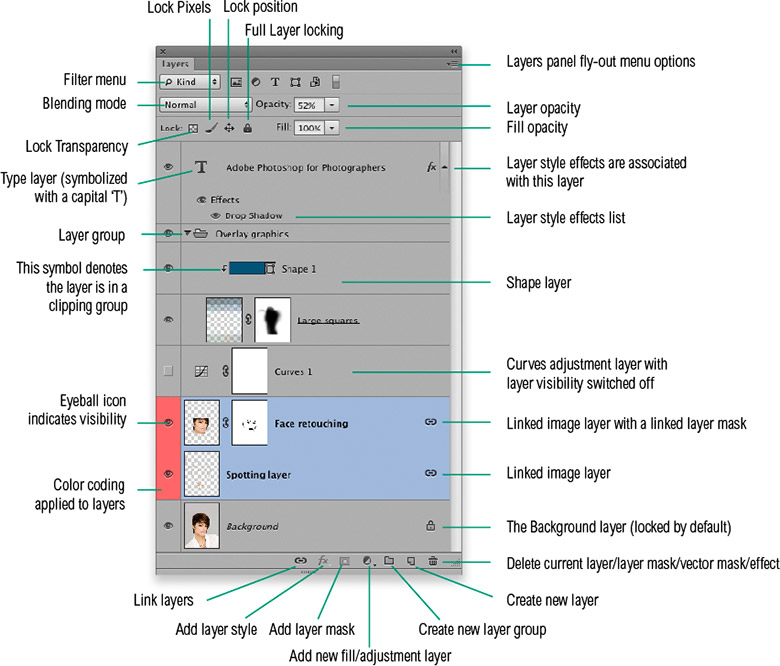
\includegraphics[width=.7\textwidth]{images/layers.jpg}
		\end{center}
	\end{frame}
	
		\subsection{Layers Tab}		
				\begin{frame}
			\frametitle{Layers Tab}
	\begin{columns}
	\column{.6\textwidth}
	\vspace{-15pt}
	\begin{outline}
		\1 Layers contain the images, text, or objects that make up a layered file. 
		\2 They let you move, edit, and work with content on one layer without affecting content on other layers.
		\1 If the Layers panel is not visible, choose Window - Layers.
		\1 A layer must be selected in order to make changes to it.  
		\1 To add more layers to your selection, hold Control as you click other layers.
	\end{outline}
	\column{.45\textwidth}
	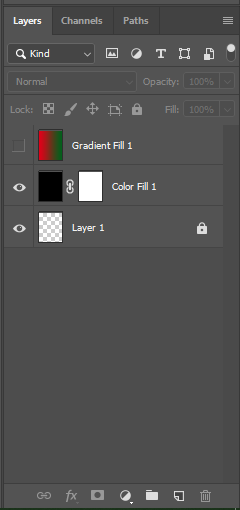
\includegraphics[width=.7\textwidth]{images/layers tab.png}
\end{columns}
		\end{frame}
	
	\subsection{Creating \& Naming Layers}		
\begin{frame}
	\frametitle{Creating a New Layer}
	\begin{itemize}
		\item Click the Create a New Layer icon at the bottom of the layers panel to make a new layer. 
		\item This layer is transparent until something is added to it.
	\end{itemize}
	\begin{center}
		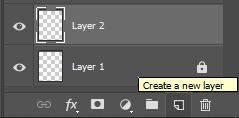
\includegraphics[width = 0.6\textwidth]{images/new layer.png}
	\end{center}
\end{frame}

\begin{frame}
	\frametitle{Renaming a Layer}
	\begin{itemize}
		\item To name a layer, double-click the current layer name. 
		\item Type a new name for the layer. 
		\item Press Enter
	\end{itemize}
	\begin{center}
		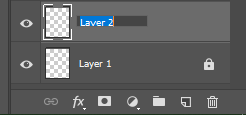
\includegraphics[width = 0.6\textwidth]{images/renaming a layer.png}
	\end{center}
\end{frame}
	
			\subsection{Stack Order \& Groups}		
	\begin{frame}
		\frametitle{Stack Order}
	\begin{columns}
	\column{.6\textwidth}
	\vspace{-25pt}
	\begin{itemize}
			\item Layers are arranged in a stack in the Layers panel, which is usually located in the bottom right of the work area.
\item Drag a layer up or down in the Layers panel to change the order of layered objects in the image.
	\end{itemize}
	\column{.45\textwidth}
			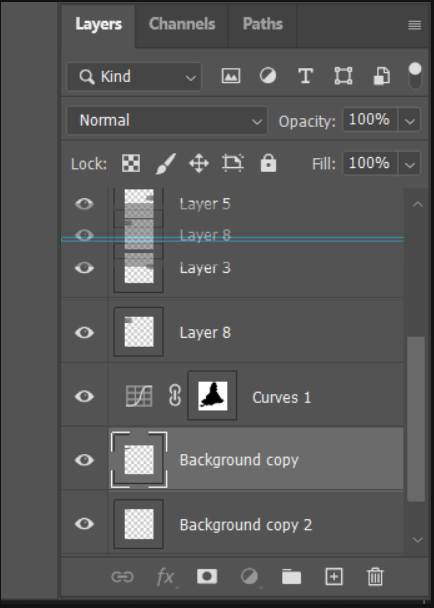
\includegraphics[width = 1.0\textwidth]{images/stack order.png}
\end{columns}
\end{frame}

\begin{frame}
	\frametitle{Groups}
	\begin{columns}
	\column{.6\textwidth}
	\vspace{-25pt}
	\begin{itemize}
		\item Groups allow you to organize your layers.
\item A new layer appears either above the selected layer or within the selected group in the Layers panel.
\item To create a layer from an existing file, Drag the file onto an open image in Photoshop.
	\end{itemize}
	\column{.45\textwidth}
		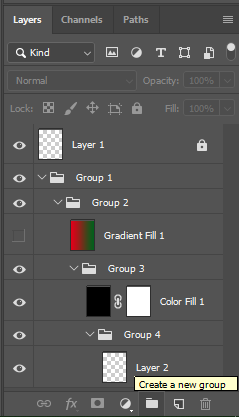
\includegraphics[width = 0.85\textwidth]{images/groups.png}
\end{columns}
\end{frame}

		\subsection{Opacity \& Fill}		
\begin{frame}
	\frametitle{Opacity}
	\begin{itemize}
		\item To change a layer’s opacity, select a layer in the Layers panel and drag the Opacity slider located near the top of the Layers panel to make the layer more or less transparent.
		\item Opacity is the extent to which something blocks light.
	\end{itemize}
	\begin{center}
		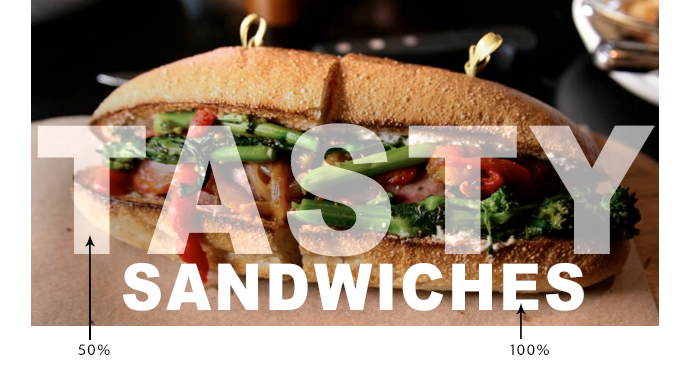
\includegraphics[width = 0.9\textwidth]{images/opacity.png}
	\end{center}
\end{frame}

\begin{frame}
	\frametitle{Fill}
	\begin{itemize}
		\item Both the Opacity and Fill options control a layer's transparency.
		\item Fill will change the transparency of any added effects (styles) to your layer, such as: stroke, drop shadow, bevel and emboss, outer glow.
	\end{itemize}
	\begin{center}
		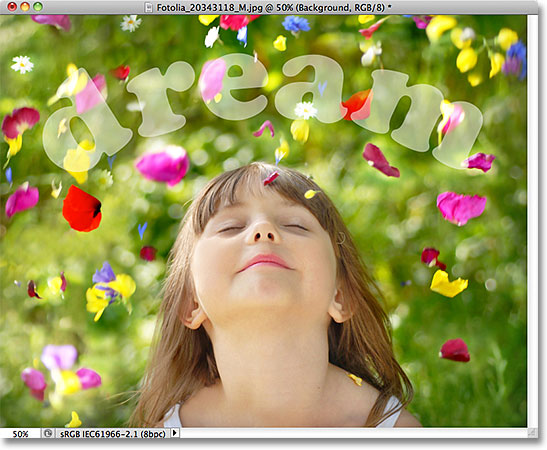
\includegraphics[width = 1.0\textwidth]{images/fill.png}
	\end{center}
\end{frame}

		\subsection{Visibility \& Locking}		
\begin{frame}
	\frametitle{Hide/Reveal}
	\begin{itemize}
		\item In the Layers panel, click the eye icon to the left of a layer to hide its content. 
		\item Click again in the same spot to reveal the content.
	\end{itemize}
	\begin{center}
		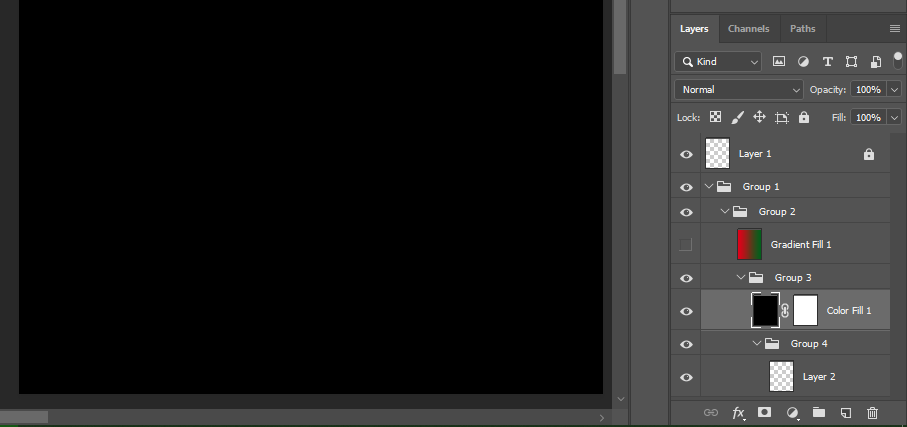
\includegraphics[width = 1.0\textwidth]{images/visibility.png}
	\end{center}
\end{frame}

\begin{frame}
	\frametitle{Locking Layers}
	\begin{itemize}
		\item You can lock layers fully or partially to protect their contents.
		\item Lock a layer to avoid making unintended changes to your work.
		\item The lock icon appears solid when the layer is fully locked and hollow when the layer is partially locked.
	\end{itemize}
	\begin{center}
		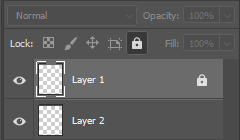
\includegraphics[width = 0.65\textwidth]{images/lock.png}
	\end{center}
\end{frame}
	
	
	\section{Move \& Zooming}
\subsection{Move Tool}
\begin{frame}
	\frametitle{Move Tool}
	\begin{itemize}
		\item The Move tool helps you position selected content or layers when customizing your work.
	\end{itemize}
	\begin{center}
		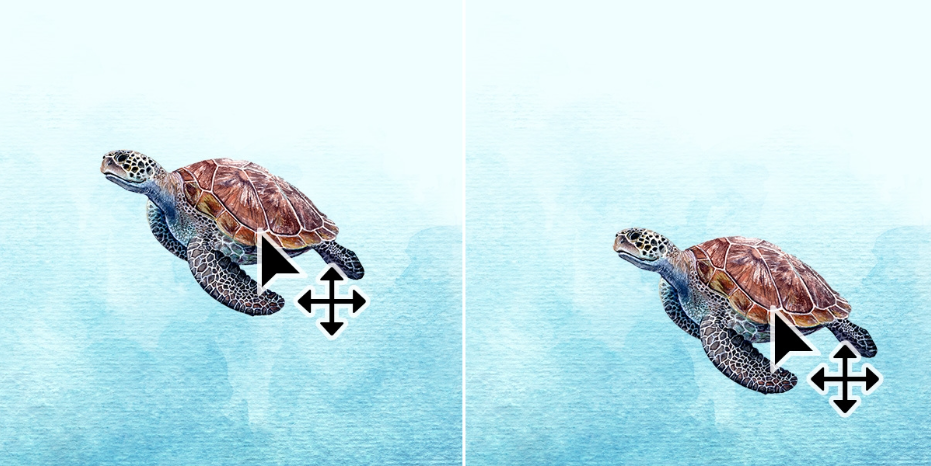
\includegraphics[width = 1.0\textwidth]{images/move tool2.png}
	\end{center}
\end{frame}

\begin{frame}
	\frametitle{Auto-Select}
	\begin{itemize}
		\item Auto-Select allows you to automatically move the selected layer wherever you click on the image.
		\item Group allows you to automatically move multiple layers together.
	\end{itemize}
	\begin{center}
		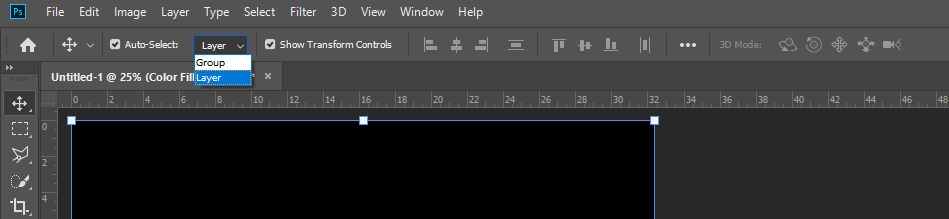
\includegraphics[width = 1.0\textwidth]{images/move tool - auto select.png}
	\end{center}
\end{frame}

\begin{frame}
	\frametitle{Transform Controls}
	\begin{itemize}
		\item Transform Controls allows you to scale the image, while moving it.
		\item Use the boxes at the corners to scale the image.
	\end{itemize}
	\begin{center}
		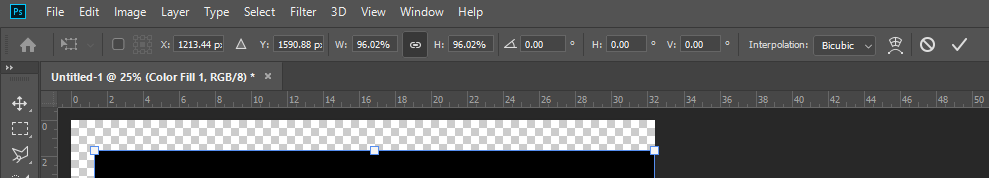
\includegraphics[width = 1.0\textwidth]{images/move tool - transform controls.png}
	\end{center}
\end{frame}

\subsection{Zoom Tool}
\begin{frame}
	\frametitle{Zoom Tool}
	\begin{itemize}
		\item Magnify or reduce the view of your image with the Zoom tool.
	\end{itemize}
	\begin{center}
		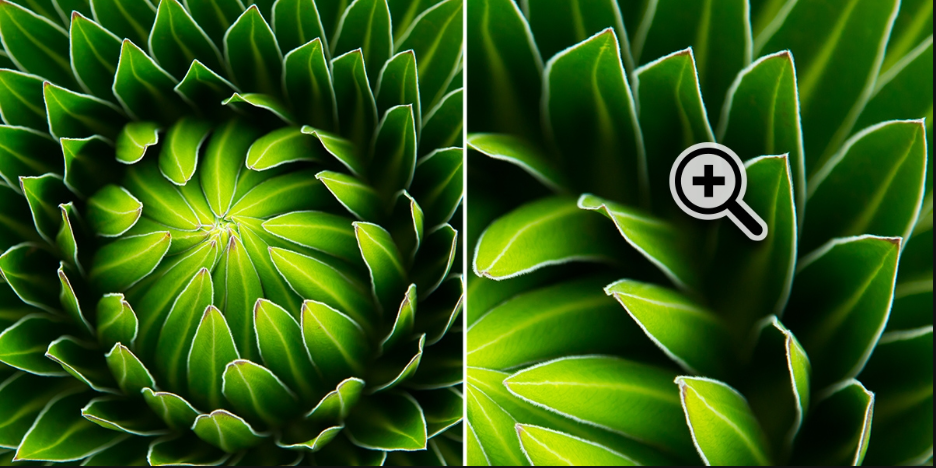
\includegraphics[width = 1.0\textwidth]{images/zoom.png}
	\end{center}
\end{frame}

\begin{frame}
	\frametitle{Scrubby Zoom}
	\begin{outline}
		\1 Click the + and - magnifying glass icons below the menu bar.
		\2 Then on the image to either zoom in or zoom out
		\1 The mouse wheel inbetween the left and right mouse buttons will scroll the window up and down.
		\2 If you hold down ctrl button, then you will scroll left and right.
		\1 Scrubby Zoom lets you zoom in and out clicking the left mouse button and holding it, then moving your mouse left and right to zoom out and in.
	\end{outline}
	\begin{center}
		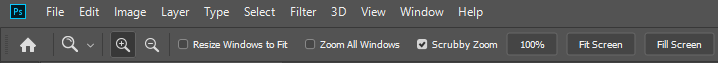
\includegraphics[width = 1.0\textwidth]{images/zoom menu.png}
	\end{center}
\end{frame}

\subsection{Hand Tool}
\begin{frame}
	\frametitle{Hand Tool}
	\begin{itemize}
		\item The Hand tool allows you to move your image while you're zoomed in to more than 100\% and part of the image is out of view.
		\item Double-click the hand tool to center the image within your current window.
	\end{itemize}
	\begin{center}
		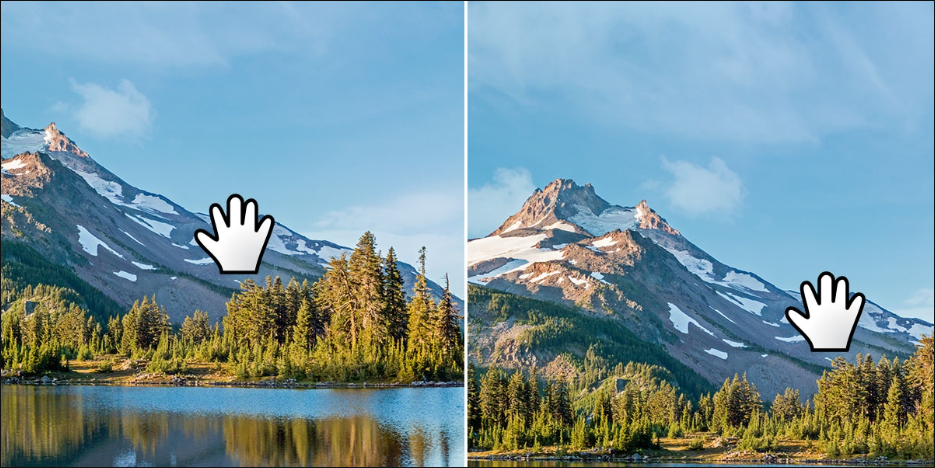
\includegraphics[width = 0.85\textwidth]{images/hand tool.png}
	\end{center}
\end{frame}

	\section{Transform}
	
		\subsection{Scale \& Rotating}
\begin{frame}
	\frametitle{Scale}
	\begin{itemize}
		\item To change the proportions of an image. For example, to make an image one-half of its original size.
	\end{itemize}
	\begin{center}
		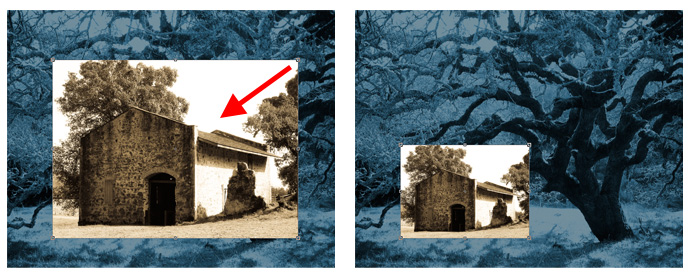
\includegraphics[width = 1.0\textwidth]{images/scale_PS.jpg}
	\end{center}
\end{frame}

\begin{frame}
	\frametitle{Content-Aware Scale}
	\begin{itemize}
		\item Content-Aware Scale resizes an image without changing important visual content such as people, buildings, animals, and so forth.
		\item While normal scaling affects all pixels uniformly when resizing an image, content-aware scaling mostly affects pixels in areas that don’t have important visual content.
	\end{itemize}
	\begin{center}
		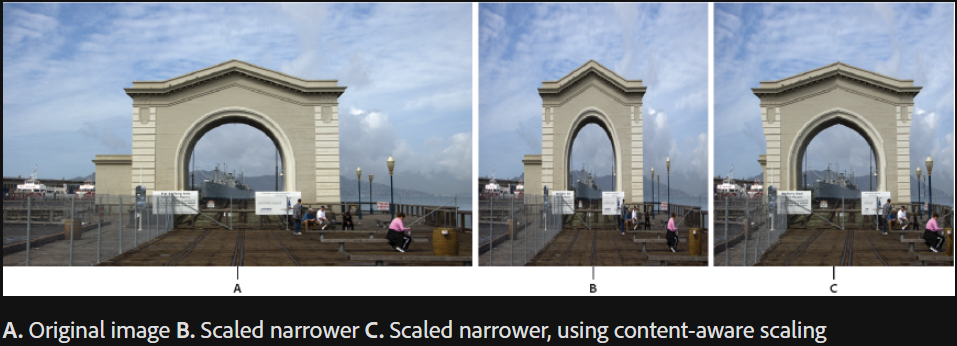
\includegraphics[width = 1.0\textwidth]{images/content aware scale.png}
	\end{center}
\end{frame}

\begin{frame}
	\frametitle{Rotate}
	\begin{itemize}
		\item To change the orientation of a selection, a layer, or an entire image (that is, the image canvas). For example, to make a vertically oriented image horizontal.
\end{itemize}
\begin{center}
	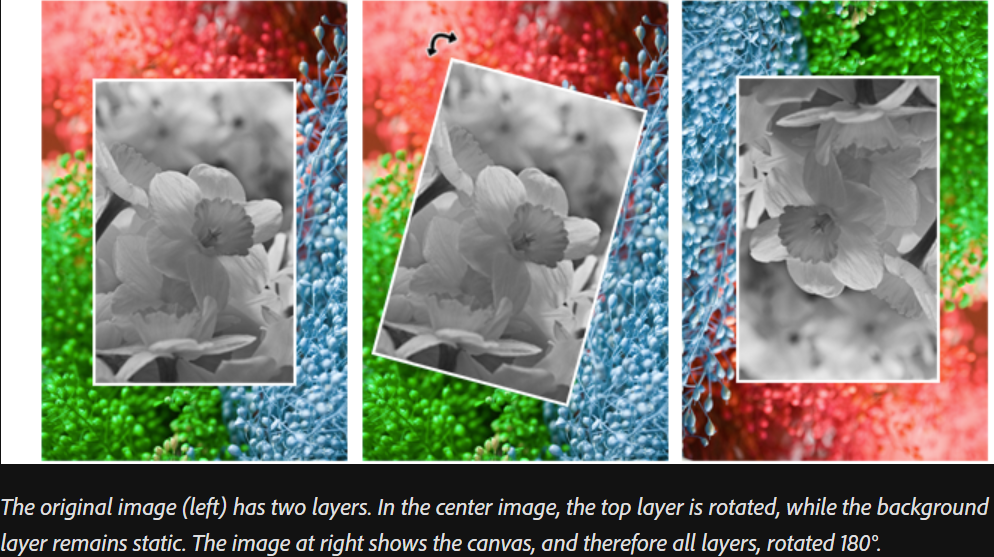
\includegraphics[width = 0.9\textwidth]{images/rotate.png}
	\end{center}
\end{frame}

\begin{frame}
	\frametitle{Rotate by Degrees}
		\begin{columns}
		\column{.6\textwidth}
		\vspace{-25pt}
	\begin{outline}
		\1 180 degrees
		\2 Rotates the entire image by rotating the top to the bottom.
		\1 90 degrees - Clockwise
		\2 Rotates the image from the top to the right.
		\1 90 degrees - Counter-Clockwise
		\2 Rotates the image from the top to the left.
\end{outline}
		\column{.45\textwidth}
		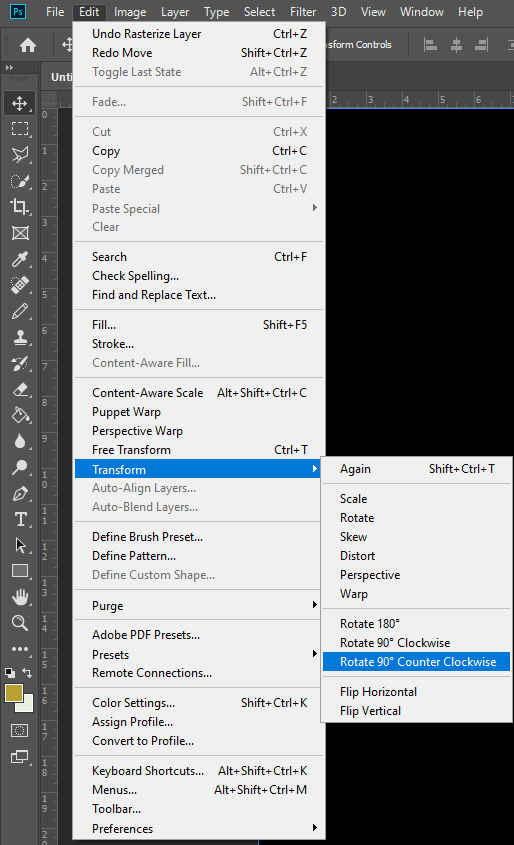
\includegraphics[width = 0.9\textwidth]{images/rotate by degrees.png}
	\end{columns}
\end{frame}

		\subsection{Skew \& Warp}
\begin{frame}
	\frametitle{Skew}
	\begin{itemize}
		\item To apply a horitzontal or vertical slant to an image.
	\end{itemize}
	\begin{center}
		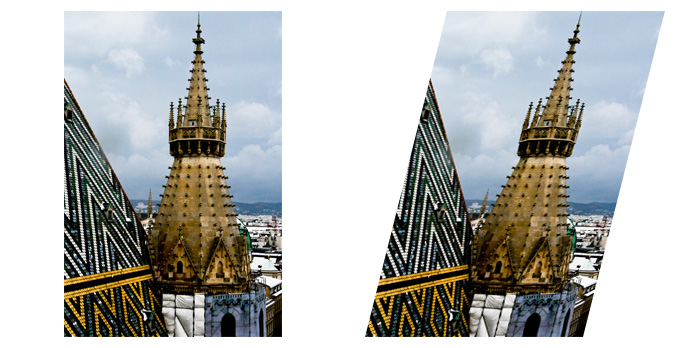
\includegraphics[width = 1.0\textwidth]{images/skew.jpg}
	\end{center}
\end{frame}

\begin{frame}
	\frametitle{Warp}
	\begin{outline}
		\1 To distort an image, often text, to conform to a variety of shapes. For instance, a line of text can be warped in the shape of an arc or wave.
		\1 How to Warp an Image:
		\2 Edit - Transform - Warp 
		\1 How to Warp Text:
		\2 Layer - Type - Warp Text
	\end{outline}
	\begin{center}
		
\includegraphics[width = 0.6\textwidth]{images/warp.png}
	\end{center}
\end{frame}

		\subsection{Distort \& Perspective}
\begin{frame}
	\frametitle{Distort}
	\begin{itemize}
		\item We are able to drag each corner in any direction separately.  
		\item Photoshop adjusts the image to fit within the new frame.
	\end{itemize}
	\begin{center}
		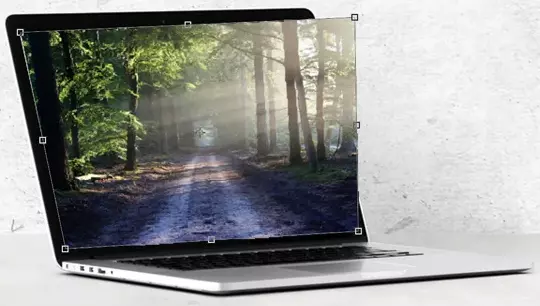
\includegraphics[width = 0.9\textwidth]{images/distort.png}
	\end{center}
\end{frame}

\begin{frame}
	\frametitle{Perspective}
	\begin{itemize}
		\item Similar to Distort
		\item Used to make text look like its tilting back towards the horizon, similar to the scrolling text at the beginning of Star Wars movies.
		\item When you draw a corner, its opposing corner will move in the opposite direction.
	\end{itemize}
	\begin{center}
		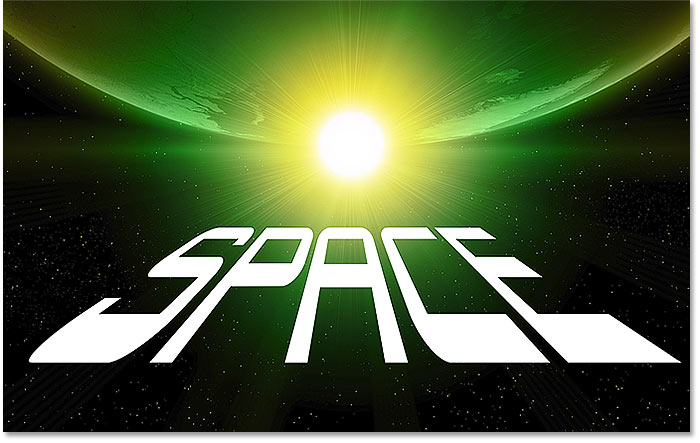
\includegraphics[width = 0.75\textwidth]{images/perspective.jpg}
	\end{center}
\end{frame}



		\subsection{Flip}
\begin{frame}
	\frametitle{Flip Horizontal}
	\begin{itemize}
		\item Flip the image from left to right.
	\end{itemize}
	\begin{center}
		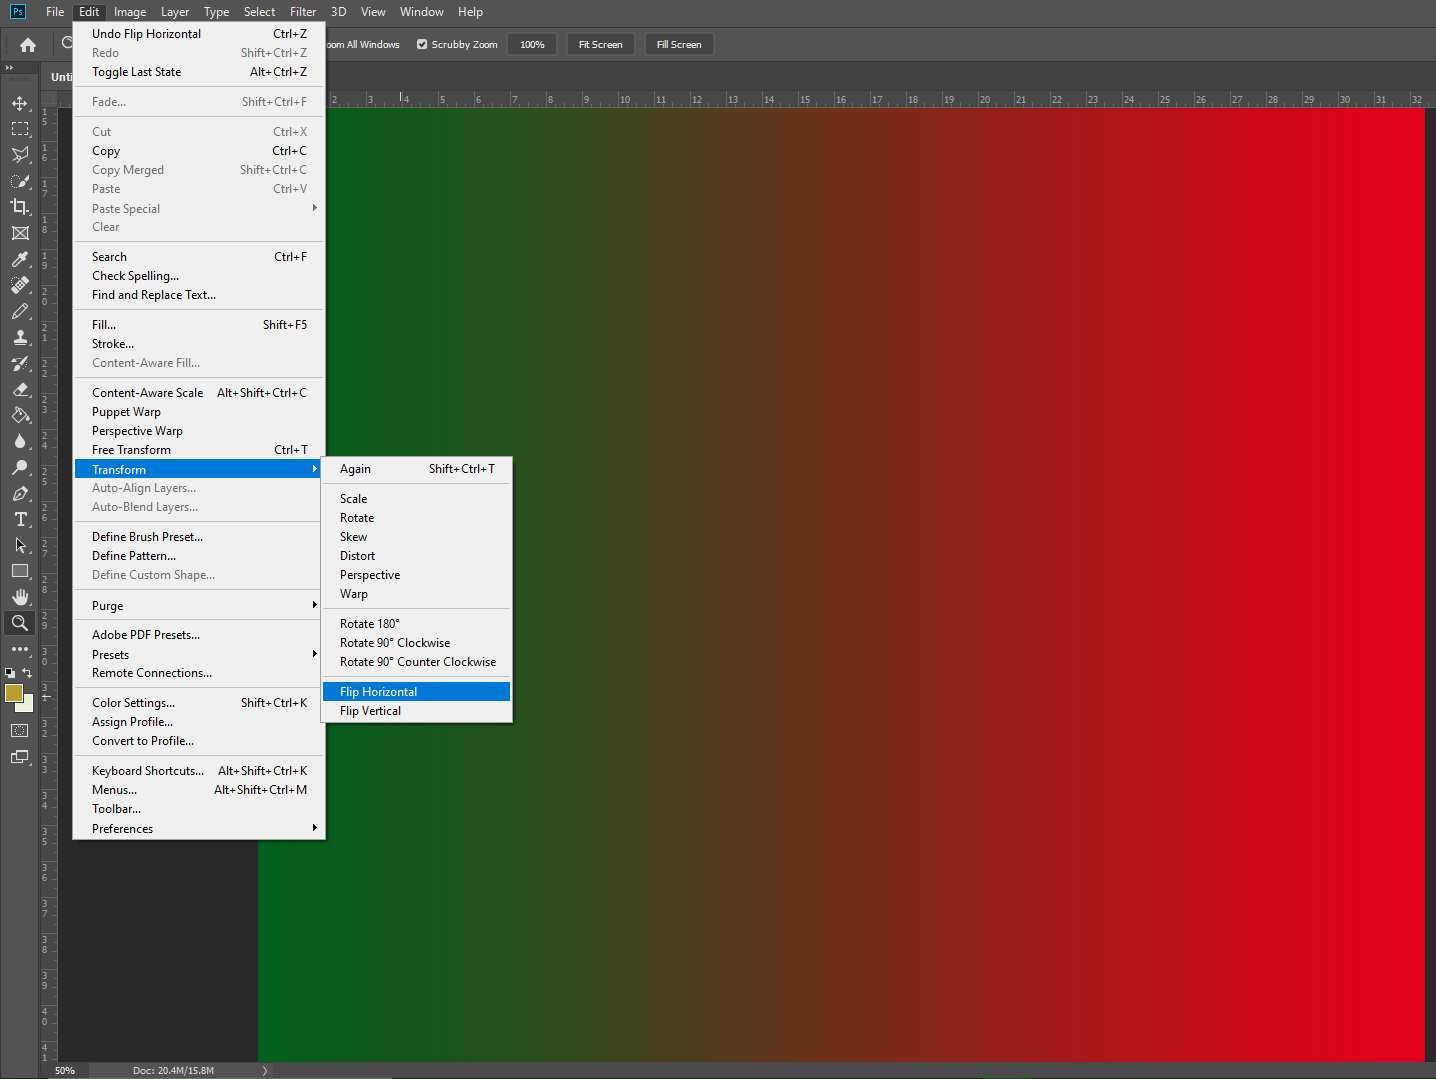
\includegraphics[width = 1.0\textwidth]{images/flip horizontal.png}
	\end{center}
\end{frame}

\begin{frame}
	\frametitle{Flip Vertical}
\begin{itemize}
	\item Flip the image from up to down.
\end{itemize}
\begin{center}
	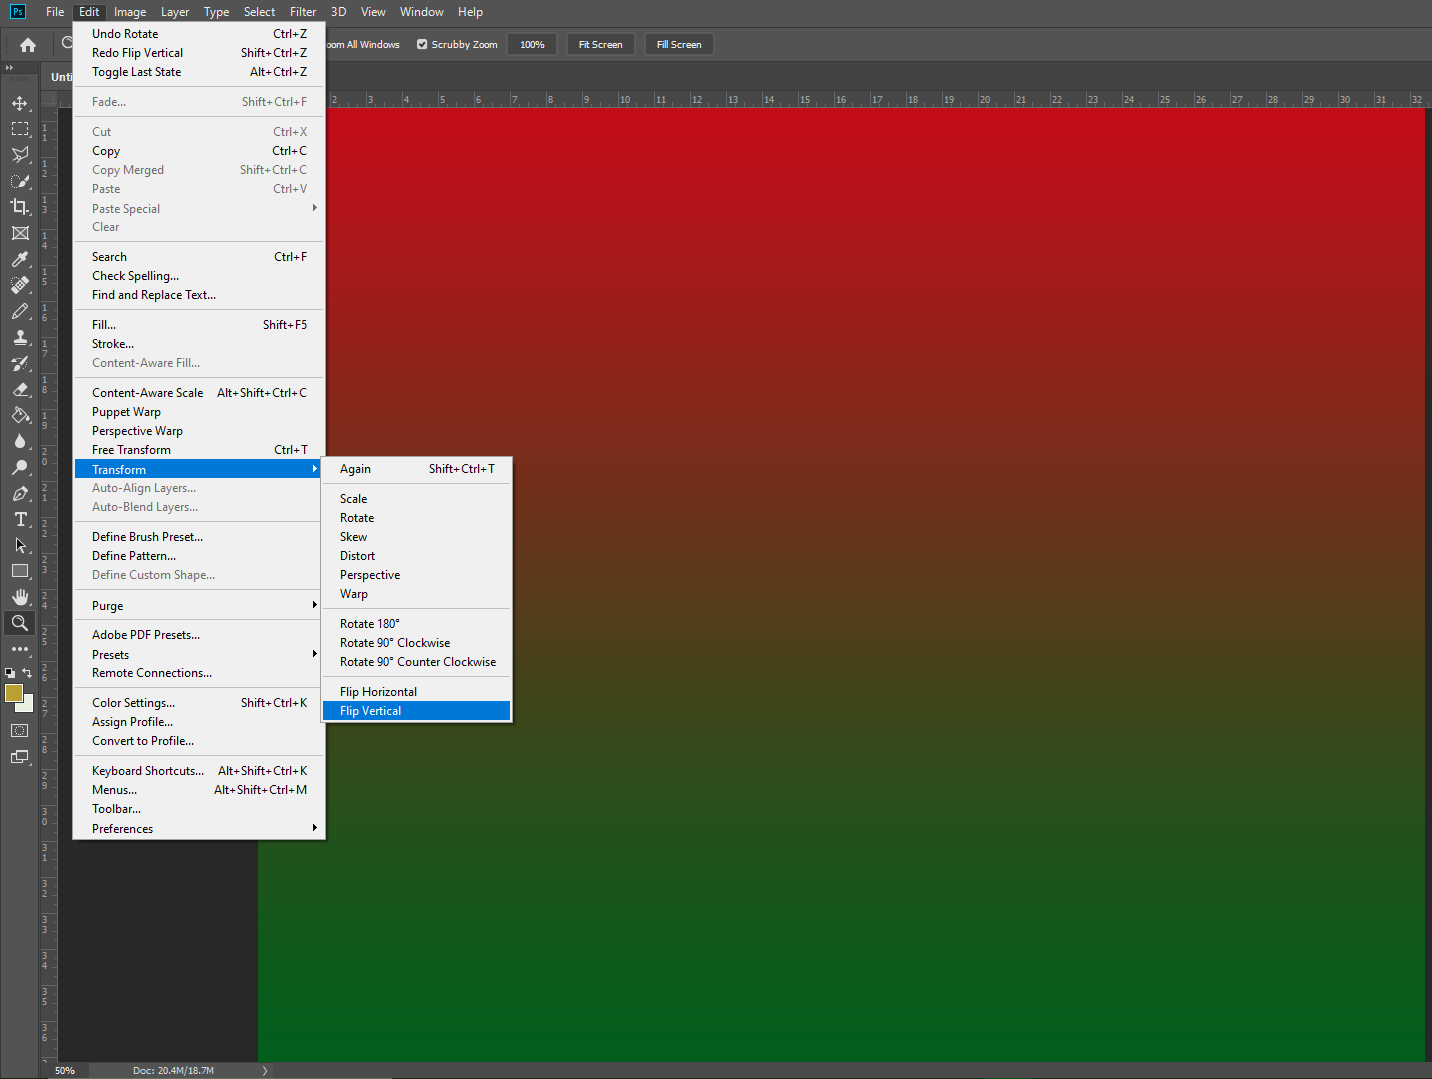
\includegraphics[width = 1.0\textwidth]{images/Flip Vertical.png}
\end{center}
\end{frame}

		\subsection{Free Transform}
\begin{frame}
	\frametitle{Free Transform}
	\begin{itemize}
		\item The Free Transform feature allows you to make several transformations at once, rather than one at a time.
		\item To use the Free Transform feature, select a layer, then choose Free Transform from then Edit menu.
	\end{itemize}
	\begin{center}
		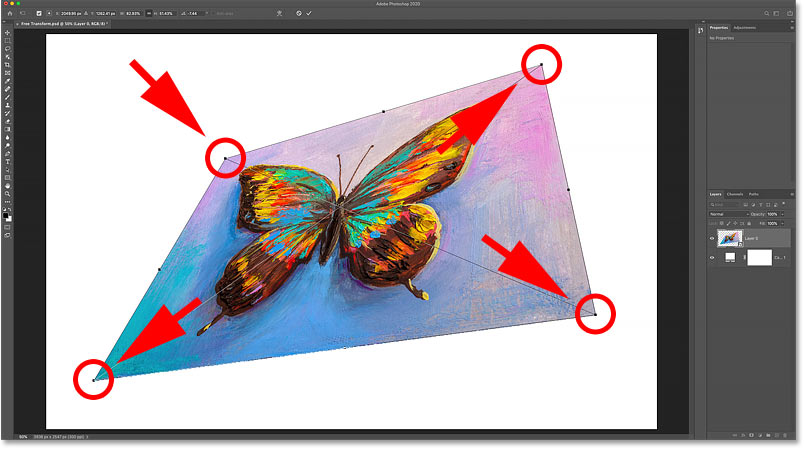
\includegraphics[width = 0.9\textwidth]{images/free transform.jpg}
	\end{center}
\end{frame}


		
		
	\section{Layer Styles}
	
	\subsection{Blending Optins}

	\begin{frame}
		\frametitle{Lossy Compression}
		\begin{outline}
			\1 Lossy Compression:
			\2 An algorithm which preserves a representation of the original uncompressed image.  
			\2 It can appear perfect to the human eye, but it is not a perfect copy.  
			\2 Lossy compression will generally produce an image with a smaller size compared to lossless compression.  
			\1 File Extension Examples:  
			\2 .jpg, .jpeg, .heif
		\end{outline}
		\begin{center}
			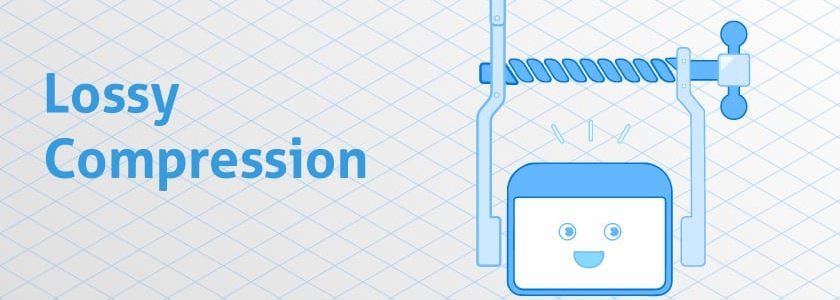
\includegraphics[width = 0.8\textwidth]{images/lossy compression.png}
		\end{center}
	\end{frame}

	\begin{frame}
	\frametitle{Lossless Compression}
	\begin{outline}
		\1 Lossless Compression:
		\2 An algorithm which reduces an images file size while preserving a perfect copy of the original uncompressed image.  
		\2 Lossless Compression will generally result in a larger file size compared to Lossy Compression.  
		\2 It is best to work with lossless files, then export a final lossy image to avoid loosing quality do to re-compression.
		\1 File Extension Examples:  
		\2 .png, .webp, .gif, .bmp
	\end{outline}
	\begin{center}
		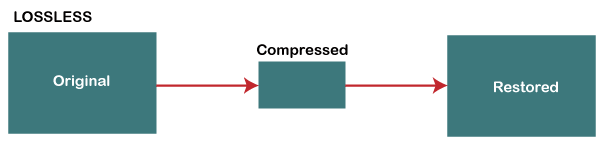
\includegraphics[width = 1.0\textwidth]{images/lossless compression.png}
	\end{center}
\end{frame}

	\begin{frame}
	\frametitle{Raw Format}
	\begin{outline}
		\1 Raw Image Format:  
		\2 Not an actual image file
		\2 Contains minimally processed data from the image sensor.
		\2 Must be processed by a raw converter to a file format such as jpg or png for displaying, printing and manipulation.
		\1 Analogous to undeveloped (or "exposed") film.  
		\1 File Extension Examples:  
		\2 .dng, .arw, .crw, .orf
		\end{outline}
	\begin{center}
		
\includegraphics[width = 0.6\textwidth]{images/raw.jpg}
	\end{center}
\end{frame}

		\begin{frame}
	\frametitle{Compression Example}
	
	\begin{center}
		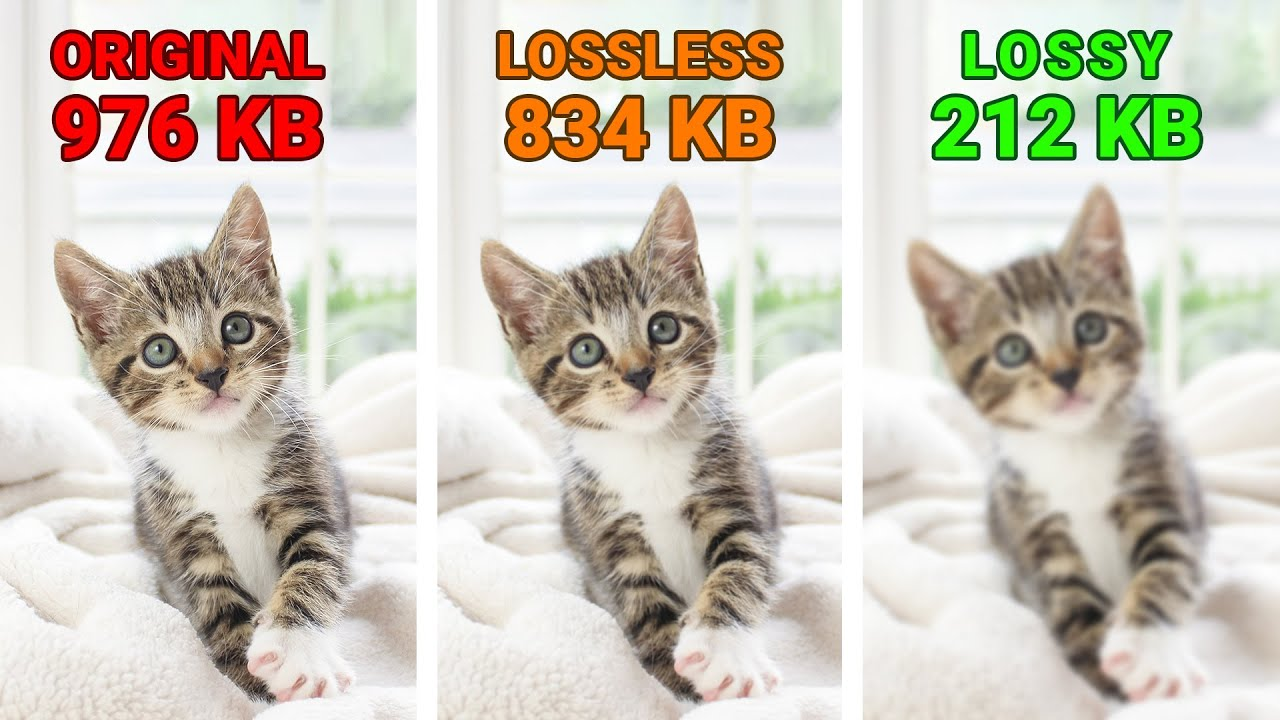
\includegraphics[width = 1.0\textwidth]{images/maxresdefault.jpg}
	\end{center}
\end{frame}

\subsection{Pixels}
\begin{frame}
	\frametitle{Pixels}
	\begin{itemize}
		\item The smallest controllable element of a picture represented on the screen.  
		\item For imaging sensors, a pixel refers to a single sensor element, in an array of elements.  Also called a sensel.  
		\item A resolution of 1920 x 1080 is 2.07MP (Megapixels)
	\end{itemize}
	\begin{center}
		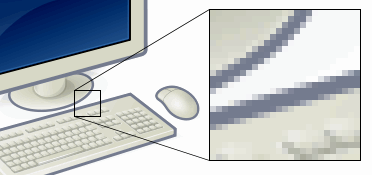
\includegraphics[width = 0.9\textwidth]{images/Pixel-example.png}
	\end{center}
\end{frame}
	
\subsection{Raster Format}
\begin{frame}
	\frametitle{Raster Graphics}
	\begin{columns}
		\column{.6\textwidth}
		\vspace{-25pt}
		\begin{outline}
		\1 Represent a two-dimensional (2D) picture as a grid of pixels.
		\1 Typically measured in width and height of pixels.  
		\1 This is what we will be working with in Photoshop.
		\1 We will always export our images as .png in this class.
		\1 File Extension Examples:  
		\2 .jpg, .png, .gif, bmp
		\end{outline}
		\column{.45\textwidth}
		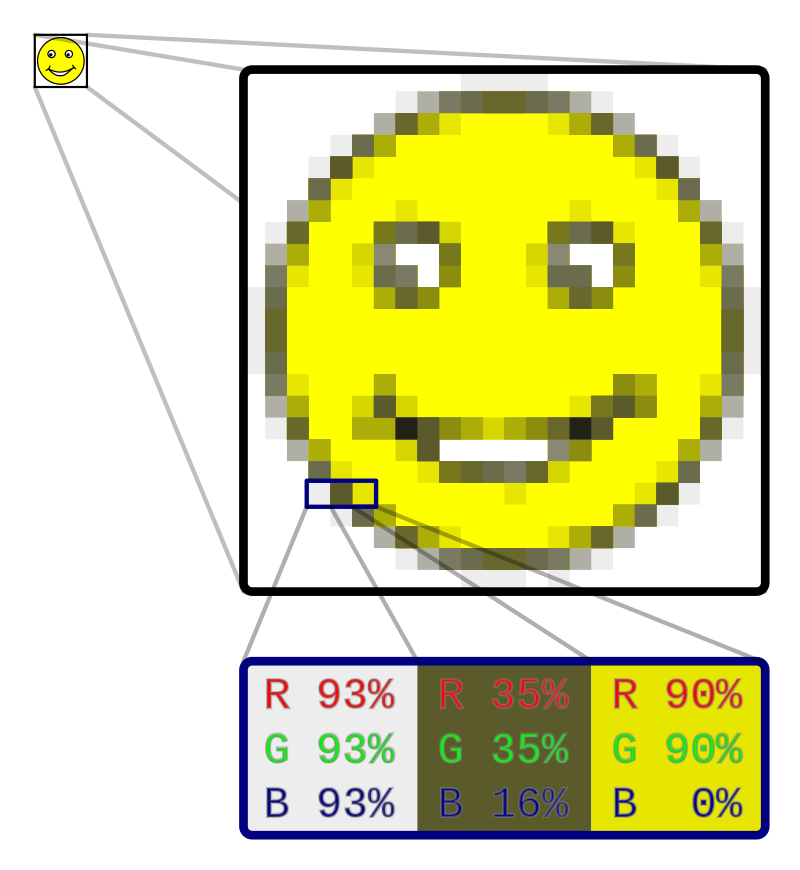
\includegraphics[width=1.0\textwidth]{images/800px-Rgb-raster-image.svg.png}
	\end{columns}
\end{frame}

\subsection{Vector Format}
\begin{frame}
	\frametitle{Vector Graphics}
		\begin{outline}
	\1 Vector graphics are based on the mathematics of analytic or coordinate geometry.  
	\1 They are scalable and offer a high degree of accuracy
	\1 Computationally intensive, as the computer must calculate and render the graphic each time.
	\1 File Extension Examples:  
	\2 .svg, .wmf, .eps, .cdr, .ai
\end{outline}
	\begin{center}
		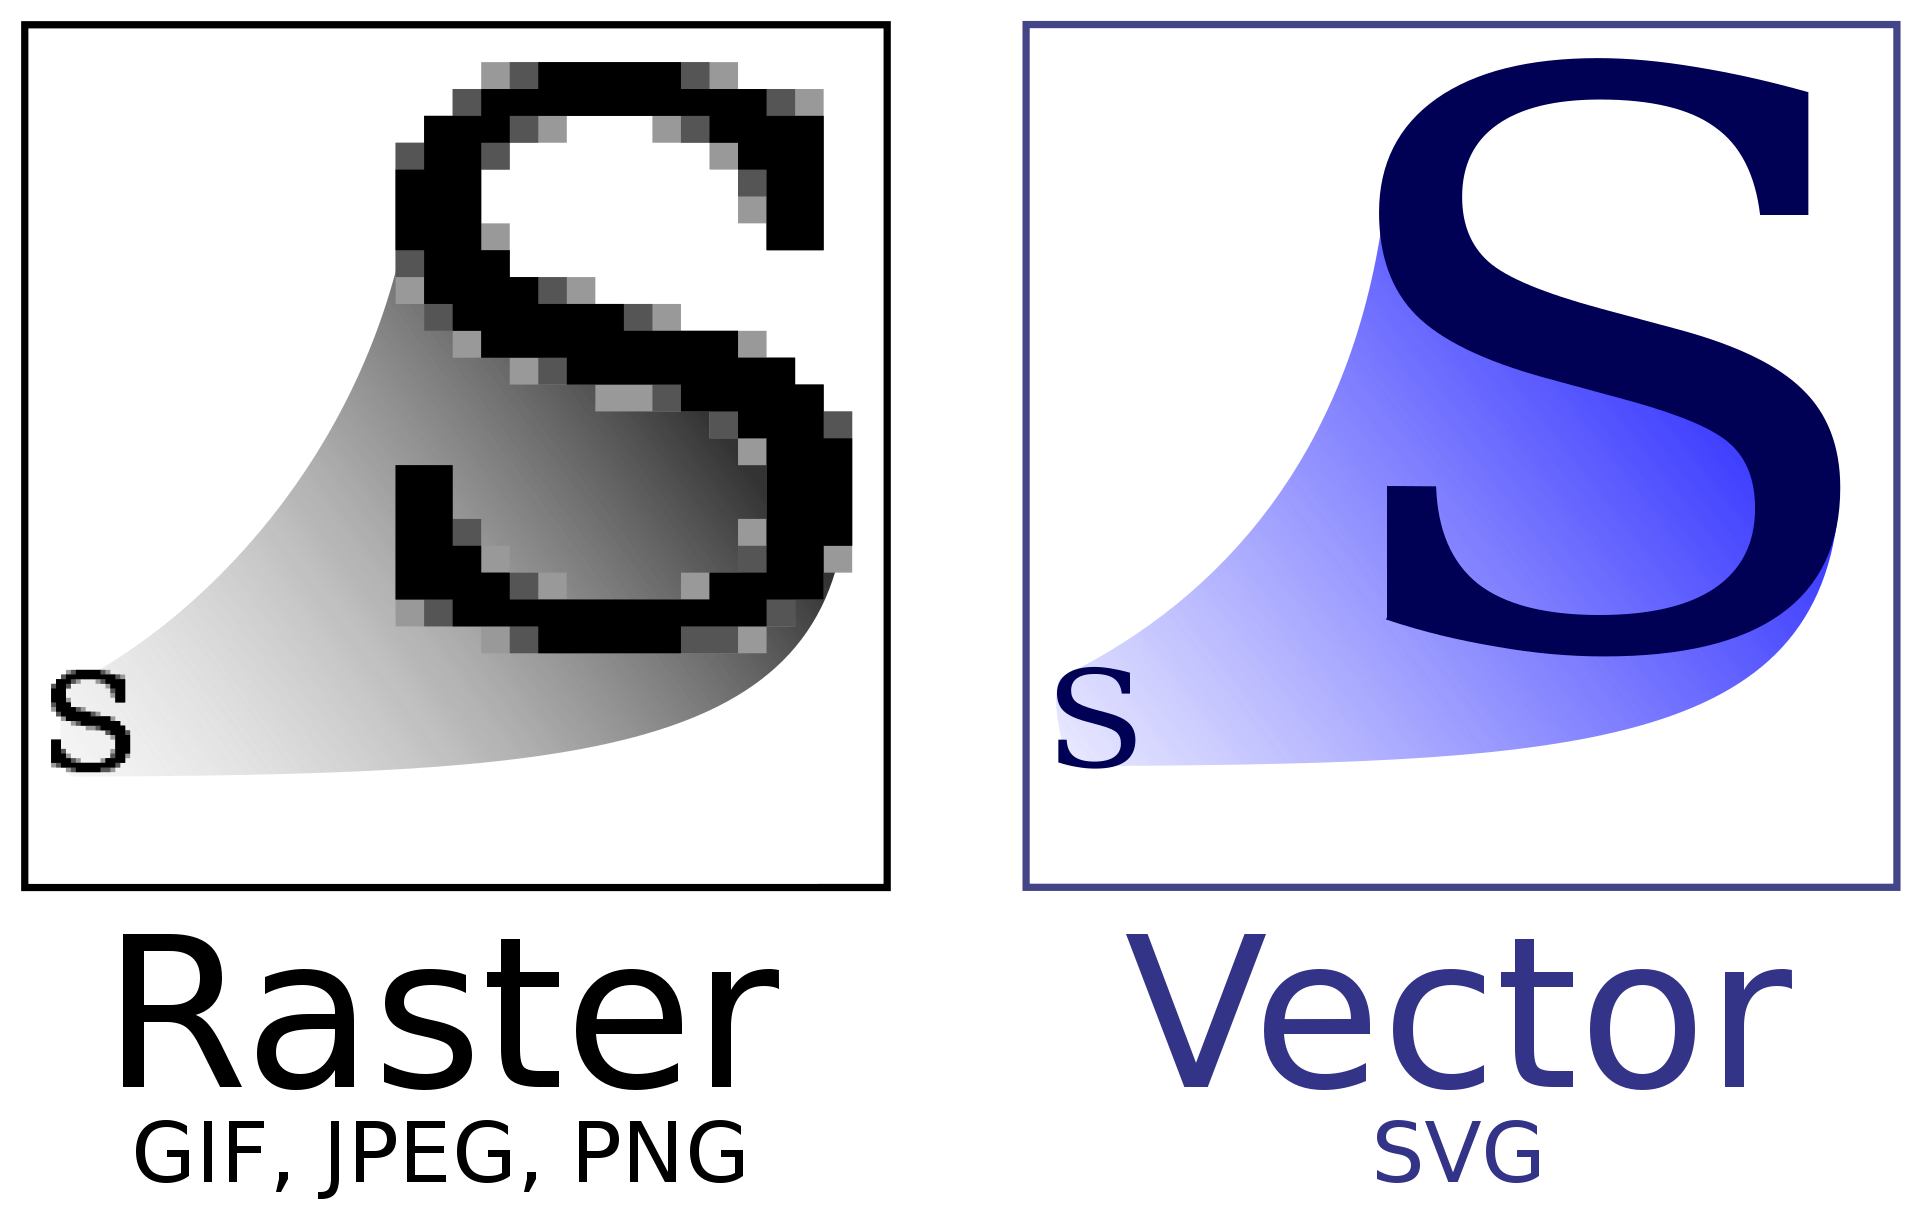
\includegraphics[width = 0.6\textwidth]{images/Bitmap_VS_SVG.svg.png}
	\end{center}
\end{frame}

\subsection{Compound Format}
\begin{frame}
	\frametitle{Container (Wrapper) Format}
	\begin{outline}
		\1 Contains both Raster and Vector graphics.  
		\1 Utilizes metadata to embed multiple streams of data into a single file.
		\1 File Extension Examples:  
		\2 .pdf, swf, eps, xaml, wmf
	\end{outline}
	\begin{center}
		
\includegraphics[width = 0.7\textwidth]{images/pdf.png}
	\end{center}
\end{frame}


	\section{Exporting Images}	
	
	\subsection{Why Export?}
	\begin{frame}
		\frametitle{Export vs Save}
		\begin{outline}
			\1 If you have only a single layer:
			\2 The Save option will save your edited image directly (potentially over-writing the original image)
			\1 If you have 2 or more layers:
			\2 The save option will save the Photoshop Project file, which contains all the layers within it.
			\3 File Extension:  .psd
			\1 Export will create a new image file based on all your visible layers.
		\end{outline}
		\begin{center}
			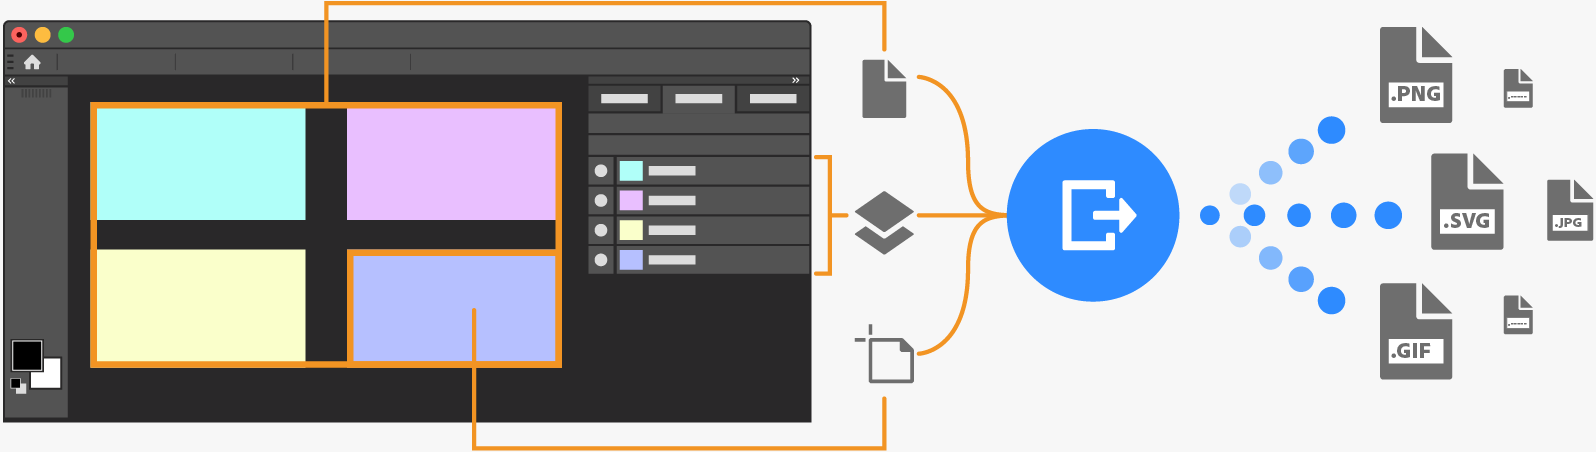
\includegraphics[width = 1.0\textwidth]{images/exporting.png}
		\end{center}
	\end{frame}

\subsection{Quick Export as PNG}
\begin{frame}
	\frametitle{Quick Export as PNG}	
	\begin{columns}
		\column{.6\textwidth}
		\vspace{-75pt}
		\begin{itemize}
			\item Fastest way to save your image.
			\item Saves a png to your default (or preset) settings.  
			\item This will usually suit your needs
		\end{itemize}
		\column{.45\textwidth}
		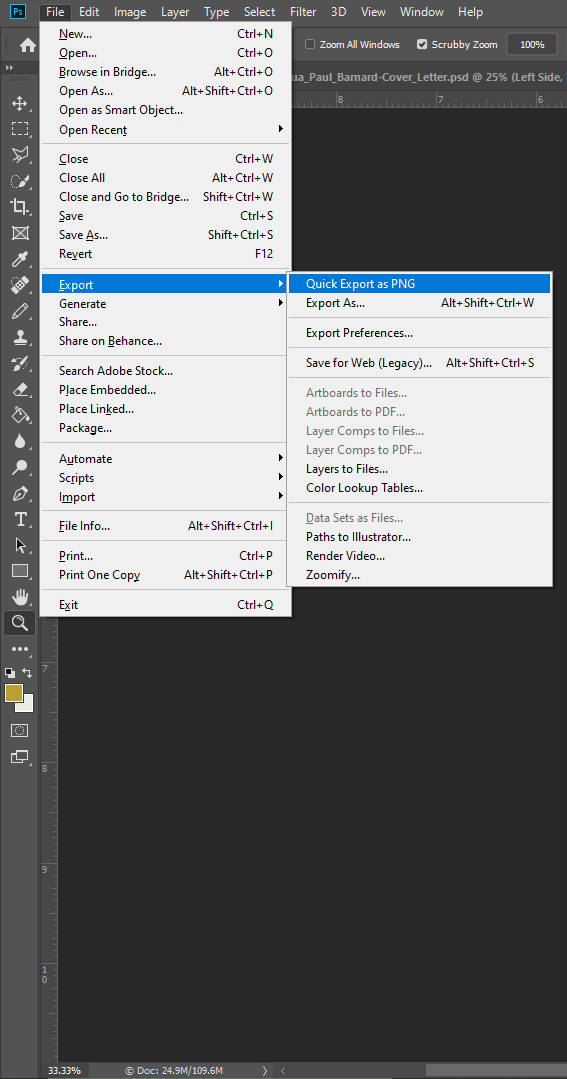
\includegraphics[width=1.0\textwidth]{images/Screenshot_5.png}
	\end{columns}
\end{frame}

\subsection{Export As...}
\begin{frame}
	\frametitle{Export As}
	\begin{outline}
		\1 The Export As option gives you way more control over your final image.
		\1 You can manually set:
		\2 Image and Canvas size (in pixels)
		\2 Scaling and Resampling Method
		\2 Transparency and bit-map
		\2 Format and Metadata
		\1 File Extension Formats available:
		\2 .png, .jpg, .gif, .svg
	\end{outline}
	\begin{center}
		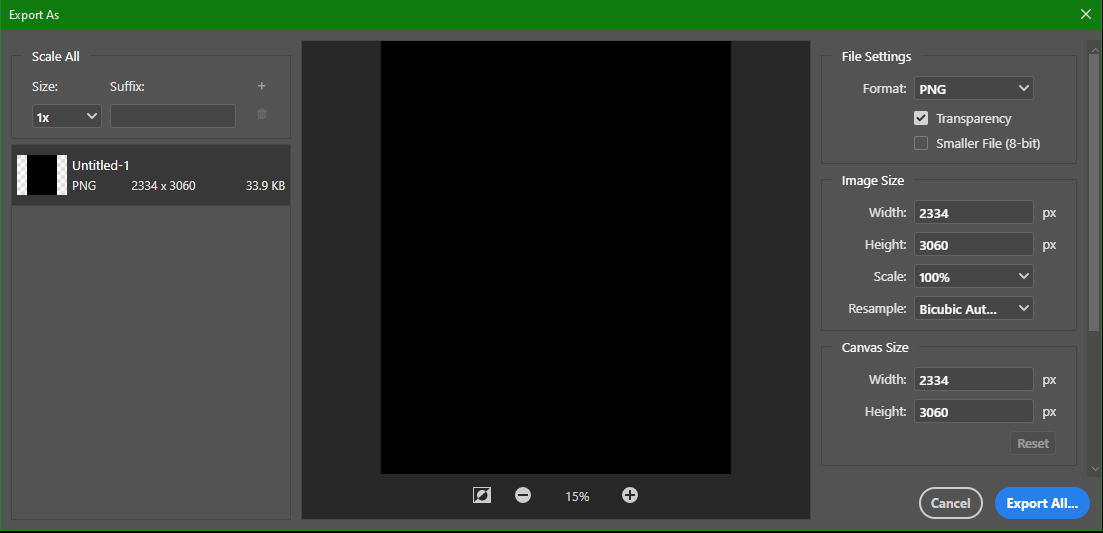
\includegraphics[width = 0.6\textwidth]{images/export as.png}
	\end{center}
\end{frame}

\subsection{Save for Web}
\begin{frame}
	\frametitle{Save for Web (Legacy)}	
		\begin{itemize}
			\item More Options than Export As...
			\item Typically used for animated gifs.
			\item Will not be used in this class.
		\end{itemize}
	\begin{center}
		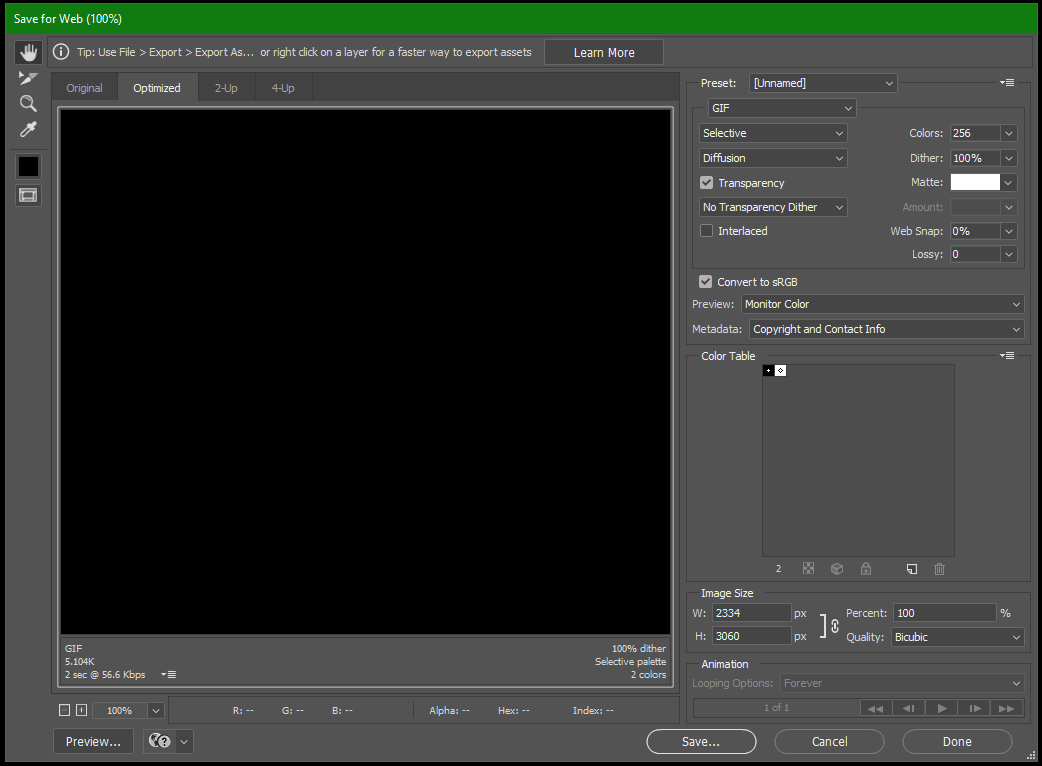
\includegraphics[width=.7\textwidth]{images/save for web.png}
		\end{center}
\end{frame}

	\section{}	
		\subsection{End Card}
	\begin{frame}
		\frametitle{End Card}	
		\begin{columns}
			\column{.6\textwidth}
			\vspace{-25pt}
			\begin{itemize}
				\item Joshua Paul Barnard
				\item Computer Science Instructor
				\item Mendocino College
			\end{itemize}
			\begin{itemize}
				\item This Presentation was made in \LaTeX
				\item For the Fall 2022 semester.  
			\end{itemize}
			\begin{itemize}
				\item jbarnard@mendocino.edu
				\item github.com/JoshuaPaulBarnard
			\end{itemize}
			\column{.45\textwidth}
			
\includegraphics[width=.85\textwidth]{images/shone farm wine pouring - vert.png}
		\end{columns}
	\end{frame}
	
\end{document}